% Include both PDFs and this fragment from the same graphics search path.
\begin{figure}[!t]
\centering
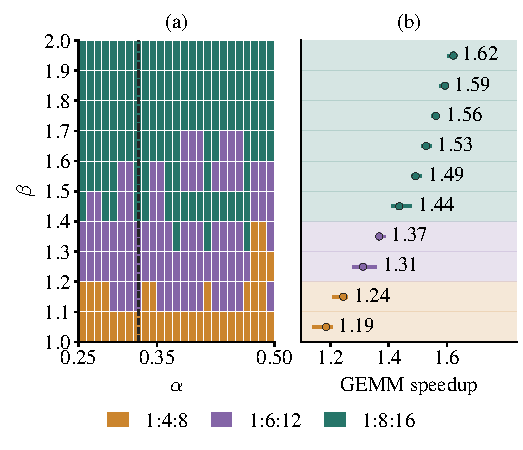
\includegraphics[width=\columnwidth]{budget_sweep.pdf}
\caption{Budget sensitivity for five equally weighted precision-migration scenarios and 2,047 first LLM requests from FreeInference agent sessions. (a) Each $0.1$-wide power-budget band is colored by the ratio attaining the lowest modeled GEMM time over the largest fraction of that band. The area fraction $\alpha$ retains its exact core-count boundaries. (b) At $\alpha=0.327$ (dashed line), each curve compares band-averaged compute time with the $1:2:4$ baseline. Thick segments mark the band winner by coverage.}
\label{fig:first_request_budget_sweep}
\end{figure}
\begin{figure}[!t]
\centering
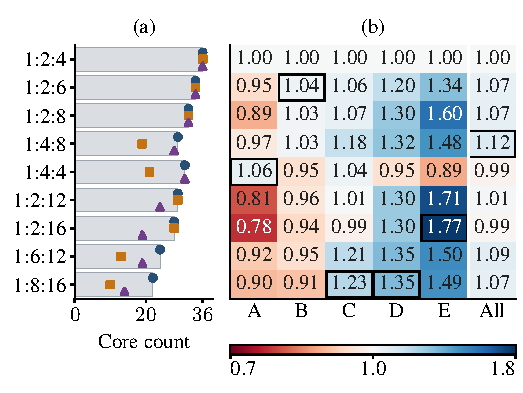
\includegraphics[width=\columnwidth]{case_32k.pdf}
\caption{Cold prefill at 32,768 input tokens, $\alpha=0.327$, and $\beta=1$. (a) Gray bars show physical cores. Circles, squares, and triangles mark active cores for BF16, MXFP8, and MXFP4, respectively. (b) Ideal GEMM compute speedup over $1:2:4$ for migration stages A--E. All compares mean times across the five stages. Outlines identify column maxima before rounding.}
\label{fig:first_request_case_32k}
\end{figure}
